\section{Pressure Regimes Are Not Universal Residency Thresholds}
\label{sec:pressure-regimes}

\begin{figure}[t]
    \centering
    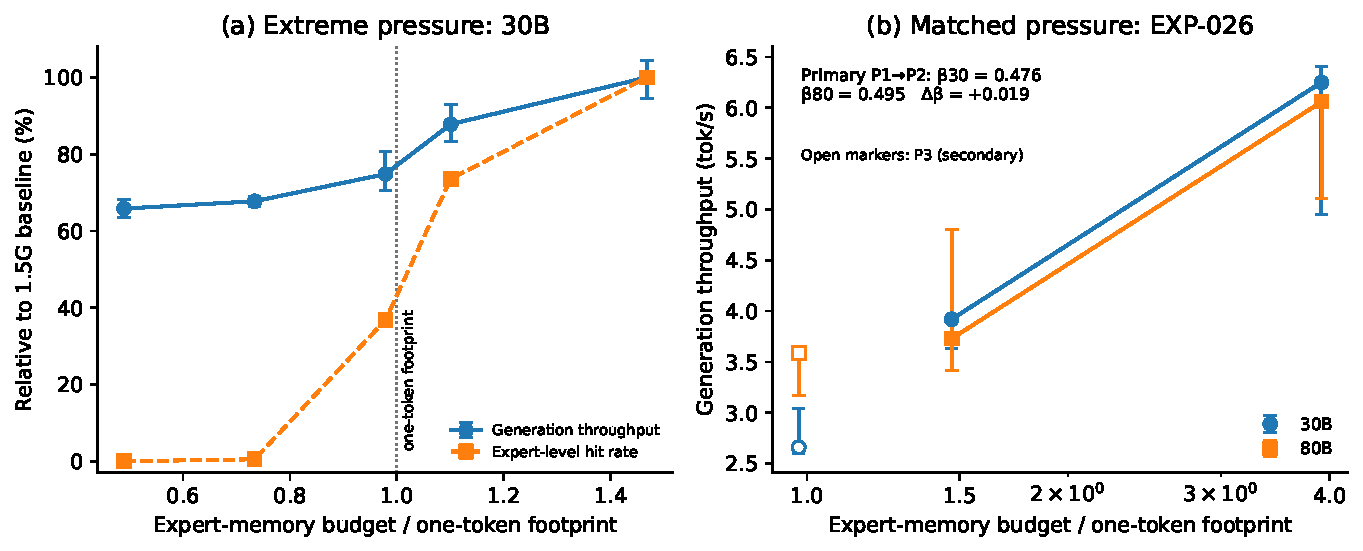
\includegraphics[width=\linewidth]{../experiments/EXP-026-30b-vs-80b-regimes/figures/cross_regime_synthesis.pdf}
    \caption{Reuse transitions and performance regimes are not universal residency thresholds. Panel (a) shows the 30B extreme-pressure result normalized to the 1.5\,GiB baseline: expert-level reuse collapses substantially faster than generation throughput, and execution continues below the one-token expert footprint. Panel (b) shows the matched-pressure comparison: the preregistered P1$\rightarrow$P2 pressure-response exponents are $\beta_{30}=0.476$ and $\beta_{80}=0.495$ ($\Delta\beta=+0.019$), so the models are not distinguished by the primary explanandum. Open markers show the secondary P3 condition.}
    \label{fig:pressure-regimes}
\end{figure}
